\documentclass[12pt]{amsart}
\usepackage{amsmath,amssymb,url,color,tikz}
\usetikzlibrary{patterns} 
\usepackage[all]{xy}
\usepackage{young}
\usepackage{enumerate}
\usepackage[margin=1in]{geometry}
\usepackage{hyperref}
\usepackage{graphicx}
\usepackage{caption} 
\usepackage{subcaption}
\usetikzlibrary{arrows,automata}
\usepackage[colorinlistoftodos,color=red!70]{todonotes}

%\oddsidemargin = 0.0cm \evensidemargin = 0.0cm \textwidth = 6.5in
%\textheight =8.5in


\newtheorem{thm}{Theorem}
\newtheorem{lem}[thm]{Lemma}
\newtheorem{prop}[thm]{Proposition}
\newtheorem{cor}[thm]{Corollary}
\newtheorem{conj}[thm]{Conjecture}
\newtheorem{qn}[thm]{Question}

\theoremstyle{definition}
\newtheorem{defn}[thm]{Definition}
\newtheorem{ex}[thm]{Example}

\theoremstyle{remark}
\newtheorem{rem}[thm]{Remark}

\numberwithin{thm}{section}


\newcommand{\IMAGE}{\text{IMAGE}}
\newcommand{\LUT}{\text{LUT}}
%\newcommand{\RR}{\mathbb{R}}
%\newcommand{\ZZ}{\mathbb{Z}}
%\newcommand{\mcO}{\mathcal{O}}

\newcommand{\minho}[1]{\todo[color=yellow,inline]{minho: #1}}
\newcommand{\doyeob}[1]{\todo[color=blue!70,inline]{doyeob: #1}}
\newcommand{\mario}[1]{\todo[color=red,inline]{mario: #1}}
\newcommand{\emily}[1]{\todo[color=gray,inline]{emily: #1}}
\newcommand{\chensu}[1]{\todo[color=orange,inline]{chensu: #1}}
\newcommand{\morgan}[1]{\todo[color=green,inline]{morgan: #1}}
\newcommand{\chaiwah}[1]{\todo[color=pink,inline]{chaiwah: #1}}

\renewcommand{\qedsymbol}{$\blacksquare$}
\def\<{\langle}
\def\>{\rangle}
\def\longto{\longrightarrow}

\begin{document}


%\title{Team 4 (Fast and Somewhat Accurate Algorithms)}
\title{Fast and Somewhat Accurate Algorithms}

\author[Barela]{Mario Barela}
%, The University of Iowa}
\author[Chen]{Su Chen}
%, University of Kansas}
\author[Gunawan]{Emily Gunawan}
%, University of Minnesota}
\author[Schreffler]{Morgan Schreffler}
%, University of Kentucky}
\author[Song]{Minho Song}
%, Sungkyunkwan University
\author[Yeo]{Doyeob Yeo}
%, Korea Advanced Institute of Science and Technology (KAIST)}
\author[Wu]{Mentor: Chai Wah Wu (IBM), Team 4}

\address{Mathematical Modeling in Industry XIX (August 5-14, 2015)}

\date{August 5-14, 2015}
%\date{\today}
\maketitle

%%=======================================
\section{Introduction and Problem Statement}
%%=======================================
In applications such as image processing, computer vision or image compression, often times accuracy and precision are less important than processing speed as the input data is noisy and the decision making process is robust against minor perturbations. For instance, the human visual system (HVS) makes pattern recognition decisions even though the data is blurry, noisy or incomplete and lossy image compression is based on the premise that we cannot distinguish minor differences in images. In this project we study the tradeoff between accuracy and system complexity as measured by processing speed and hardware complexity.
\emily{This paragraph above is exactly what Chai wrote in the IMA page, so we probably need to paraphrase it.}

We seek to produce algorithms using look-up-tables (LUT) for speeding up filter operations (such as edge-detection, sharpening, blurring, and embossing filters). In order for any LUT-based algorithm to be useful, the size of the LUTs need to be reasonably small. To meet this aim, we use the following strategies.
\begin{enumerate}
\item a byte-truncation technique, 
\item convolution decompositon of a kernel $3\times 3$ matrices (rank one),
\item approximate convolution decompositon of a kernel $3\times 3$ matrices (rank two)
\item and taking advantage of the observation that edge-detection algorithm shows higher tolerance to byte-truncation. 
\end{enumerate}

\section{Background}

\cite{WSLQE06} discusses fast algorithms using look-up tables (LUT).



An $h$-by-$w$-pixel image file can be thought of as a three-dimensional array $\IMAGE = \left[p_{ijk}\right]_{h\times w\times 3}$ whose entries are integers between 0 and 255. Given pixel $(i,j)$, the three entries $p_{ijk}$, $k=1,2,3$, determine the color of the pixel in some colorspace. When the image is grayscale, let $\IMAGE = [p_{ij}]_{h\times w}$, and let the entries indicate the pixel's intensity (0 for black, 255 for white). For the sake of simplicity, we will only consider grayscale images in this paper.

\subsection{Filtering images using kernel convolutions}

When filtering an image, first choose a matrix $K = [k_{ij}]_{n\times n}$ with double-precision entries, where $n$ is an odd number greater than 1. The matrix $K$ is called the \emph{filter kernel} or \emph{convolution kernel}. In this paper we usually only consider $3\times3$ and $5\times5$ kernels.

Next, we compute the \emph{matrix convolution} $F = K * \IMAGE$,  a $\max\{h,n\}\times\max\{w,n\}$ matrix whose $ij$th entry is
\[f_{ij} = \begin{cases}
\displaystyle\sum_{q = (1-n)/2}^{(n-1)/2}\sum_{r = (1-n)/2}^{(n-1)/2}k_{i+q,j+r}p_{i-q,j-r} & \textrm{if } 1\le i+q \le h,\ 1 \le j+r \le w\\
\hspace{2cm} 0 & \textrm{otherwise}.
\end{cases}\]
To eliminate the piecewise nature of determining $f_{ij}$, one can first ``pad'' $\IMAGE$ with a frame of zeros that is $\frac{n-1}{2}$ entries thick. Observe that this definition of matrix convolution coincides with the usual discrete convolution, but with two-dimensional indexing instead of one-dimensional. In particular, it is associative and distributive.

\subsection{Truncation methods}

Recall that the value of a pixel is an integer between $0$ and $255$, which is an 8-bit number. Given an $n\times n$ filter kernel $K$, we say that $T= [t_{ij}]_{n\times n}$ is a \emph{truncation matrix} if its entries are all integers between 0 and 8. When performing a kernel convolution on an $n\times n$ block $\IMAGE_B$ of $\IMAGE$, $T$ indicates that we ignore (or truncate) the last $t_{ij}$ bits of the $ij$th entry of $\IMAGE_B$ when applying $K$. 

\subsection{Measures of errors}

\emily{Chai suggested we run through a suite of images, for example, maybe the images from the Kodak website, and confirm that the errors are similar.}

\begin{defn}
Given two images $A=[a_{ij}]_{h \times w}$ and $B=[b_{ij}]_{h \times w}$, we will define $\ell^2$-difference$(A,B)$ and $\ell^\infty$-difference$(A,B)$ by 
\begin{align*}
\ell^2\text{-difference}(A,B) &:= \sqrt{ \frac{ \sum_{i,j} \left( a_{ij} - b_{ij} \right)^2} {h \times w}},\ \textrm{and}\\
\ell^\infty\text{-difference}(A,B) &:= \textrm{max}_{i,j} \left \vert a_{ij} - b_{ij} \right\vert.
\end{align*}

The PSNR (in dB) \cite{wikipedia/PSNR} is defined as
\begin{displaymath}
\begin{array}{ccl}
\textrm{PSNR}(A,B) & = & 10\cdot \textrm{log}_{10} \left( \frac{\textrm{MAX}_B^2}{\textrm{MSE}} \right)\\
		 & = & 20 \cdot \textrm{log}_{10} \left( \frac{\textrm{MAX}_B}{\sqrt{\textrm{MSE}}} \right)
\end{array}
\end{displaymath}
where
\begin{displaymath}
\textrm{MSE} = (\ell^2\text{-difference}(A,B))^2 \qquad \textrm{and} \qquad \textrm{MAX}_B= 255.
\end{displaymath}
\end{defn}

\begin{rem}
In general, $\text{MAX}_B$ is the maximum \emph{possible} pixel value of an image. Since we are assuming each pixel is an 8-bit integer, $\text{MAX}_B$ will be 255 for our purposes.
\end{rem}

\begin{rem}
PSNR can be easily calculated by using MATLAB command $\textrm{psnr}(A,B)$.
PSNR is the abbreviation for Peak Signal-to-Noise Ratio. In brief, it shows us how different two images are. As PSNR is higher, it becomes harder to recognize the difference between original image and filtered image. Typical values for the PSNR in lossy images are between 30 and 50 dB, provided the bit depth is 8 bits. 
\end{rem}

\begin{defn}
The \emph{Image Euclidean Distance (IMED)} is given by
\[d_\text{IMED}^2(A,B) = \frac{1}{2\pi}\sum_{i,k = 1}^h\sum_{j,\ell = 1}^w \exp\left(\frac{-(k^2+\ell^2)}{2}\right)\big(a_{ij}-b_{ij}\big)\big(a_{i+k,j+\ell} - b_{i+k,j+\ell}\big).\]
\end{defn}
\begin{rem}
See \cite{FWZ05} for an analysis of why IMED might be a reasonable image distance. Another reasonable image distance may be $\frac{d_\text{IMED}}{\sqrt{h\cdot w}}$.
\end{rem}

\section{Challenges}
On Wednesday August 5, we
decided that look-up tables  are not suitable for a median filter algorithm.

Although high-pass filters seem to respond well to truncation, blurring filter does not respond well to truncation.

\section{Results}

\subsection{Truncation and Look-up tables (without decomposition)}

\subsubsection{A High-pass kernel}

\subsubsection{Sobel Magnitude Operation}
$\mathbf{G} = \sqrt{ {\mathbf{G}_x}^2 + {\mathbf{G}_y}^2 }$

where

$\mathbf{G}_x = \begin{bmatrix} 
 -1 & 0 & +1  \\
-2 & 0 & +2 \\
-1 & 0 & +1 
\end{bmatrix} * \mathbf{A}
\quad
\mbox{and}
\quad   
\mathbf{G}_y = \begin{bmatrix} 
-1 & -2 & -1 \\
 0 & 0 & 0 \\
+1 & +2 & +1
\end{bmatrix} * \mathbf{A}$.

Here $*$ denotes the 2-dimensional convolution operation.

Let $K_x=\begin{bmatrix} 
 -1 & 0 & +1  \\
-2 & 0 & +2 \\
-1 & 0 & +1 
\end{bmatrix}$.
A full look-up table $\LUT(K_x)$ for $K_x$ requires $256^6$ bytes to store. In contrast, a look-up table $\LUT(K_x)(T)$ with truncation matrix $T= \begin{bmatrix} 
5 & 8 & 5 \\
 5 & 8 & 5 \\
5 & 8 & 5
\end{bmatrix}$ takes up $8^6$ bytes.

Let $\mathbf{G}(T)$ denote the Sobel magnitude operation using the truncated look-up table $\LUT(K_x)_T$.
For images in our test suite,
the PSNR values between $\mathbf{G}$ and $\mathbf{G}(T)$ range between $25$ and $31$.

\begin{table}[ht]
\begin{center}
\begin{tabular}{c|c|c|c|}\cline{2-4}
& $\mathbf{G}-\mathbf{G}(T_5)$ & $\mathbf{G}-\mathbf{G}(T_4)$ & $b$ \\\hline \multicolumn{1}{ |c| }{PSNR}
& 42.0500  & 71.0895 &  \\\hline
\multicolumn{1}{ |c| }{$l_{2}$ - error}  & 0.0079 & 2.7895e-04 &  \\\hline \multicolumn{1}{ |c| }{$max$ - error} & 0.0144  & 6.1630e-04 & \\
\hline
\end{tabular}
\caption{Comparison of errors for the Sobel magnitude with a $5$-digit truncation}
\label{table:sobel}
\end{center}
\end{table}

\begin{center}
\begin{table}
	
    \begin{tabular}{ | c | c | c |   }
    \hline
    LUT Size & Best Truncation & PSNR (dB) \\ \hline
    16Kb& $00$ & 30.4442 \\ \hline
    32Kb& $(0,b,0)$ with $b=(3,3,3)^T$ & 33.3275 \\ \hline 
    256Kb& $(0,b,0)$ with $b=(2,2,2)^T$ & $00$ \\ \hline 
    \end{tabular}
    \bigskip
    
    \caption{Sobel}
\end{table} 
\end{center}

% \begin{center}
% \begin{table}
	
%     \begin{tabular}{ | c | c | c | c | c |}
%     \hline
%     LUT Size & Truncation matrix & PSNR (dB) & $\ell_2$ & $\ell_\inf$ \\ \hline
%     16Kb& $(0,b,0)$ with $b=(4,2,4)^T$ & 30.4442 & 00 & 00 \\ \hline
%     32Kb& $(0,b,0)$ with $b=(3,3,3)^T$ & 33.3275 & 00 & 00\\ \hline 
%     64Kb& $(0,b,0)$ with $b=(3,2,3)^T$ & 35.5597 & 00 & 00\\ \hline 
%     1MB& $\begin{bmatrix}
%     5 &4 & 5
%     \end{bmatrix}$ & $[29.7,33.5]$ & $[4.7 10^{-6},5.9 10^{-5}] \times 255$ & $0.09,0.12 \times 255$\\ \hline 
%     \end{tabular}
%     \bigskip
    
%     \caption{Best truncation scheme for fixed-size LUT (for Sobel magnitude operation)}
% \end{table} 
% \end{center}


\emily{
Not finished yet.
I will add the range of errors from the image test suite. 
[26.5950]    [25.8214]    [31.0469]    [30.6689]
    [30.4290]    [29.6926]    [26.5178]    [29.1399]    [28.4675]    [27.9392]

  Column 7

    [27.9151]
}

Range of $\ell_2$-difference between $10^{-5}$ and $8\, \, 10^{-6}$ (multiplied by 255).

Range of $\ell_2$-difference between $0.1100$ and $0.21$ (multiplied by 255).

\emily{Some temporary notes for my reference.

ell2 = 

    [6.7367e-06]    [7.3328e-06]    [1.0568e-05]    [7.8146e-06]


ellinf = 

    [0.1158]    [0.1213]    [0.2084]    [0.1204]}

\subsection{Decomposing rank 1 matrix}
\chensu{high-pass filter}
\emily{Sobel gradient filter}

\subsection{Approximate decomposition of a rank 2 matrix}
\mario{Approximate decomposition of a rank 2 matrix}

\subsection{Decomposing a Kernel Matrix by Rows}

Let $K$ be an $n\times n$ filter kernel. For $k=1,\ldots,n$, let $e_k$ be the $n\times 1$ matrix whose $k1$th entry is 1 and whose other entries are 0, and let $r_k$ be the $1\times n$ matrix whose entries are the $k$th row of $K$. Note that $K$ may always be decomposed as $K = \sum_{k=1}^nr_k * e_k$. Taking advantage of the associativity of $*$, it follows that $K * P = \sum_{k=1}^nr_k * \left(e_k * P\right)$. This is just another way of writing that summation is distributive, i.e.,
\[\sum_{q = (1-n)/2}^{(n-1)/2}\sum_{r = (1-n)/2}^{(n-1)/2}k_{i+q,j+r}p_{i-q,j-r} = \sum_{q = (1-n)/2}^{(n-1)/2}\left(\sum_{r = (1-n)/2}^{(n-1)/2}k_{i+q,j+r}p_{i-q,j-r}\right).\]

If using lookup tables to compute a matrix convolution, this observation greatly reduces the amount of memory required. Indeed, rather than having a single LUT which takes $n^2$ inputs and contains $2^{8n^2}$ entries, we have $n$ LUTs (one for each row of $K$), each of which takes $n$ inputs and contains only $2^{8n}$ entries. Even when $n=3$ this is a tremendous saving of memory (with 8-bit entries, one 4-zebibyte ($2^{72}$) LUT versus three 16MB ($2^{24}$) LUTs).

Further, the multiple-LUT approach can be easily implemented, and at a lower cost than direct computation. Before filtering any pixels, rotate $K$ by $180^o$ about its center. Then, take an $n\times n$ submatrix $P_{\mathrm{temp}}$ of $P$ centered about the pixel to which you wish to apply the kernel. Now simply enter the $i$th row of $P_{\mathrm{temp}}$ into the LUT associated with $r_i$ for $i = 1,2,\ldots,n$, and add the results. Thus, if we make the naive assumption that lookups and additions are computationally equivalent, only $2n-1$ operations ($n$ lookups and $n-1$ additions) are required per pixel. Compare this to $n^2+2n-2$ operations ($n^2$ multiplications and $2(n-1)$ additions) per pixel using direct computation.

Finally, when combined with bit truncation, each LUT can be made even smaller at the cost of an extra $n^2$ truncation operations per pixel. Unfortunately, if truncation is assumed equivalent to lookups and additions, this is not much more efficient than direct computation, since it saves only one operation per pixel. 

As an example, choose an arbitrary $3\times 3$ kernel $K$ and a truncation matrix $T = \left[\begin{smallmatrix}5 & 5 & 5\\5 & 2 & 5\\ 5 & 5 & 5\end{smallmatrix}\right]$, using the $i$th rows of $K$ and $T$ to produce the $i$th LUT. The associated LUTs will have 512, 4096, and 512 entries. Even if each entry uses double precision, only 20kB of memory is required to store the LUTs, which is certainly small enough to fit into cache memory. However, 14 operations (5 to use the LUTs as described previously, and 9 truncations) are required per pixel, versus 13 for direct computation. 

\subsection{Using the truncating technique for a blurring filter: Taking advantage of the fact that truncating works better for edge-detecting than for blurring}
\todo{Write a sentence here.}

\begin{rem}\label{rem:sharpening_vs_blurring}
\begin{enumerate}
\item The truncation method $T$ can be used to reduce running time.
\item Truncation introduces too much error for blurring, but is decent for edge-detecting.
\end{enumerate}
\end{rem}

Let $I$, $L$, and $H$ denote the identity, a low-pass filter operation, and a high-pass filter operation on an image.
Let $L(T)$, and $H(T)$ denote $L$ and $H$ with a truncation using the truncation matrix $T$.
To informally say that applying a truncation technique to a high-pass filter gives close enough result, we can write $H \approx H(T)$.

Since $I = L + H$, we have
$L = I - H \approx I - H(T)$.

\begin{ex}
Consider a high-pass filter
$H=
\frac{1}{8}
\begin{bmatrix}
0 & -1 & 0\\
-1 & 4 & -1\\
0 & -1 & 0
\end{bmatrix}$.
Let $$
T_{1}=\left[
\begin{array}{ccc}
8 & 4 & 8 \\
4 & 2 & 4 \\
8 & 4 & 8
\end{array}
\right] ,T_{2}=\left[
\begin{array}{ccc}
8 & 5 & 8 \\
5 & 3 & 5 \\
8 & 5 & 8
\end{array}
\right] \mbox{ and }T_{3}=\left[
\begin{array}{ccc}
8 & 6 & 8 \\
6 & 4 & 6 \\
8 & 6 & 8
\end{array}
\right]
$$
be truncation matrices. The table \ref{table:comparison_of_errors} shows us how $L(T_i)$ and $I-H(T_i)$ are different from the low-pass filter $L=I-H$ for each $i$. $L(T_i)$ is Old and $I-H(T_i)$ is New in the table \ref{table:comparison_of_errors}.

\begin{table}[ht]
\begin{center}
\begin{tabular}{c|c|c|c|c|c|c|}
\cline{2-7}  & \multicolumn{2}{|c|}{$T_{1}$} &
\multicolumn{2}{c|}{$T_{2}$} & \multicolumn{2}{c|}{$T_{3}$}
\\\cline{2-7} & Old & New & Old & New & Old & New \\\hline \multicolumn{1}{ |c| }{PSNR} &
38.12 & 39.58 & 30.80 & 32.84 & 22.59 & 25.59 \\\hline
\multicolumn{1}{ |c| }{$l_{2}$ - error} & 3.06 &  2.80 &  7.40 & 5.87 &
18.87 & 13.52 \\\hline \multicolumn{1}{ |c| }{$l_{\infty
}$ -
error} & 8.42 & 7.40 & 19.64 & 15.81 & 43.35 & 35.70 \\
\hline
\end{tabular}
\bigskip

\caption{Comparison of errors}
\label{table:comparison_of_errors}
\end{center}
\end{table}
As you see, our new approach gives us the better results no matter which truncation matrix you use.
See also Figures \ref{fig:comp} made via the truncation matrix $T_3$.
\begin{figure}[h] \centering 
\begin{subfigure}[b]{0.3\textwidth} 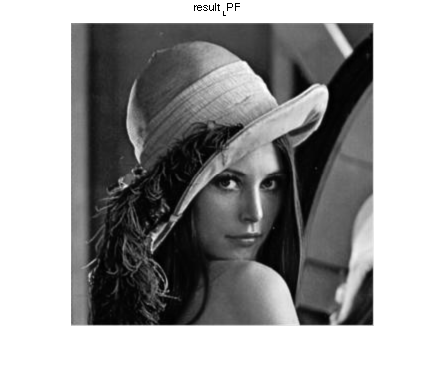
\includegraphics[width=\textwidth]{LPF.png} \caption{LPF} \label{fig:LPF} \end{subfigure}
\begin{subfigure}[b]{0.3\textwidth} 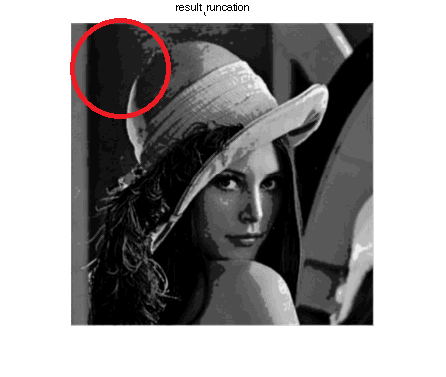
\includegraphics[width=\textwidth]{truncation.png} \caption{LPF with Truncation} \label{fig:LPF with Truncation} \end{subfigure}
\begin{subfigure}[b]{0.3\textwidth} 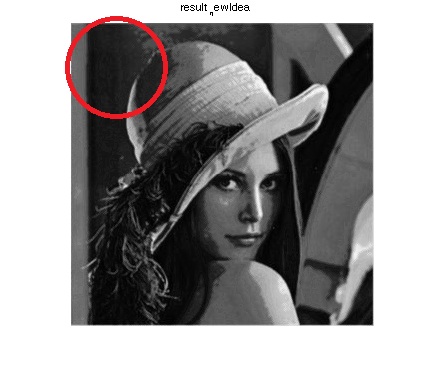
\includegraphics[width=\textwidth]{new.png} \caption{Result of the New Idea} \label{fig:new} \end{subfigure}
\caption{Comparison of filtered images}\label{fig:comp} 
\end{figure}

As you see, you can easily check that our new idea reduces staircase effects against the usual truncation method.
\end{ex}

Likewise, we can apply our method to any other low-pass filter as follows:

\begin{itemize}
\item[1.] Let $L$ be the our target low-pass filter.
\item[2.] Set $\tilde{H}:=I-L(T)$ for a certain truncation $T$.
\item[3.] Find $\tilde{L}:=I-\tilde{H}$ as an approximation of $L$.
\end{itemize}

Note that the second and third step stands for avoiding staircase effects.


\subsection{Approximate Decomposition}




\subsection{A rank 1 decomposition}
The usage of look up tables (LUTs) provides a way to reduce the implementation time caused by direct algebraic computations. By storing the values of convolution of all possible square matrices with the kermel matrix $K$, the look up table serves as a dictionary whose values can be retrieved readily. The potential challenge for LUTs lies in the size which can be so large that storing them in the computer memory become impracticle. As an example, for a $3\times 3$ kernel $K$ with all entries non-zero will require $S=(2^8)^9=2^{72}$ bytes storage, which is fall beyond the storing capability of modern computers. 
$$
\begin{bmatrix}
x_1 & x_2 & x_3\\
x_4 & x_5 & x_6\\
x_7 & x_8 & x_9
\end{bmatrix}
*
\begin{bmatrix}
k_1 & k_2 & k_3\\
k_4 & k_5 & k_6\\
k_7 & k_8 & k_9
\end{bmatrix}
\longrightarrow
\begin{bmatrix}
y_1 & y_2 & y_3\\
y_4 & y_5 & y_6\\
y_7 & y_8 & y_9
\end{bmatrix}
$$
A remedy to this problem is to use truncated versions of the LUTs. Namely, we drop a prescribed number of bits from the entries in the square matrix that will be convolved with the kernel. As an illustration, a binary number $11111011$ will become $11111000$ after we drop the last two digits, i.e. replacing them by $0$'s. In this case, the original set $\{0,1,\dots,255\}$ is turned into the set $\{0,4,8,12,\dots,252\}$ after the truncation by two bits.

Although the above truncation is able to reduce the size of LUTs substantially, it is still not enough to generate LUTs which is acceptable in practice, especially for LUTs constructed for low pass filter with 5 by 5 or even larger kernel. To deal with this issue, we introduce the decomposition of the kernel so that the LUTs for each decomposition matrix is small enough to be generated and stored in the memory. 

We first examine the simple case when $rank(K)=1$ where $K\in \mathbb{R}^{n\times n}$ and $n$ is an odd number. It is well known that every rank 1 matrix can be decomposed as
\[K=b\cdot c^T\]
for some $b,c\in \mathbb{R}^{n\times 1}$. Denoting the matrix convolution by $*$, the following relationship can be verified directly: 
\[K=b\cdot c^T=b*c^T\]
So is the equation
\begin{equation}\label{decomposition}
Image*K=Image*(b\cdot c^T)=K*(B*C)=(K*B)*C
\end{equation}
Here $B=(0,\dots,b,\dots,0)$ and $C=(0,\dots,c,\dots,0)$ where $0$ represents $n\times 1$ column vectors and $b$,$c$ are in the center. We need to point out that the above relationship may not be true for general kernel which is not rank one. This decomposition allows us to build two LUTs for the kernel $K$, each of which is a table of the column vector $b$ or $c$ since we can ignore all $0$'s. The size of LUTs are reduced significantly in this way.

As an example, let us consider the following low pass filter kernel
$$
K=\frac{1}{16}
\begin{bmatrix}
1 & 2 & 1\\
2 & 4 & 2\\
1 & 2 & 1
\end{bmatrix}
$$
It is apparent that $rank(K)=1$ and an obvious decomposition of $K$ is given by 
$$
K=\frac{1}{4}
\begin{bmatrix}
0 & 1 & 0\\
0 & 2 & 0\\
0 & 1 & 0
\end{bmatrix}*\frac{1}{4}
\begin{bmatrix}
0 & 0 & 0\\
1 & 2 & 1\\
0 & 0 & 0
\end{bmatrix}\triangleq B*C
$$
The symmetric decomposition of $K$ ($C=B^T$), simplifies the LUT further: only one LUT is required, since
\[Image*C=Image^T*B\]
The normalizing constant $\frac{1}{4}$ rules out the possibility of overflow and the maximum size (no truncation) of the LUT is $(2^8)^3=2^{24}$ bytes, or 16MB. Truncation will further reduce the size to magnitude of kilobyte. Numerical test is given in subsection 8.3. 
\subsection{Singular value decomposition}
Notice that the relationship (\ref{decomposition}) does not hold for general matrix $K$ even if $K$ can be decomposed as $K=B\cdot C$. However, it is well known that any matrix can be written as the sum of a series of rank 1 matrices, i.e. we have the following singular value decomposition (SVD): 
\[K=\sum_{i=1}^{r}\sigma_i u_i\cdot v_i^T\]
Here $u_i$,$v_i\in\mathbb{R}^{n\times 1}$ are the left and right singular vectors respectively and $\sigma_m$ are singular values. Moreover, $u_i$'s and $v_i$'s compose of orthonormal matrices and $r$ is the rank of $K$. Now we are able to make use of the LUTs for rank 1 decomposition as in the previous section. As a result, at most $2r$ LUTs are required, each of which has a maximum size of $(2^8)^n=2^{8n}$ bytes. For example, a 3 by 3 kernel with rank 2 needs at most 4 LUTs with maximum size of 16Mb for each. The benefit of SVD is that for most kernels in practice, their rank (usually 1 or 2) is far less than their dimension so that very few LUTs are required even if the kernel has large dimensions. The other benefit we obtain from SVD lies in the fact that all the summands can be dealt with independently so that the power of parallel computation can be exploited. 
\subsection{Numerical test}
In this section, we implement the ideas in 8.1 and 8.2 and perform two numerical tests. We first examine the kernel
$$
K_1=\frac{1}{16}
\begin{bmatrix}
1 & 2 & 1\\
2 & 4 & 2\\
1 & 2 & 1
\end{bmatrix}
=
\frac{1}{4}
\begin{bmatrix}
0 & 1 & 0\\
0 & 2 & 0\\
0 & 1 & 0
\end{bmatrix}*\frac{1}{4}
\begin{bmatrix}
0 & 0 & 0\\
1 & 2 & 1\\
0 & 0 & 0
\end{bmatrix}\triangleq B*C
$$
As mentioned above, one LUT need to be generated for kernel $K_1$. Some of the filtered images together with the original one ($267\times 188$) are given in figure 2. The truncation scheme $T_1$ and $T_2$ are given by 
$$
T_1=
\begin{bmatrix}
0 & 2 & 0\\
0 & 1 & 0\\
0 & 2 & 0
\end{bmatrix}
,\ \ \ \ \ \ T_2=
\begin{bmatrix}
0 & 4 & 0\\
0 & 2 & 0\\
0 & 4 & 0
\end{bmatrix}
$$
where the numbers in matrices $T_1$ and $T_2$ are those of the bits to be truncated. It is apparent in figure \ref{fig:motor} that the blurred effect with truncated LUTs for darker parts of the image is close to that from from direct application of the filter. There are visible artifacts for lighter parts of the image in the filtered images with truncated LUTs, which is an indication of a loss of precision after truncation. To measure the error introduced by our approximation, we will exploit the peak signal-to-noise ratio (PSNR) introduced in section 2. A comparison is summarized in Table \ref{tbl:low_pass}. The PSNRs for LUTs with $T_1$ and $T_2$ indicates that both schemes provides satisfactory approximation of the original filter. It is quite notable that even with truncation $T_2$, the PSNR is still above 30 with the size of LUT reduced to only 16Kb. 

We also run an optimization to examine which truncation scheme will give the best approximation of the original kernel, provided that the size of LUT is fixed. Some of the results are summarized in Table \ref{tbl:optimization}. It is not surprising that there is a symmetry in the best truncation scheme thanks to the symmetry of our original kernel $K_1$ . 

\begin{figure}[h] \centering 
\begin{subfigure}[b]{0.4\textwidth} 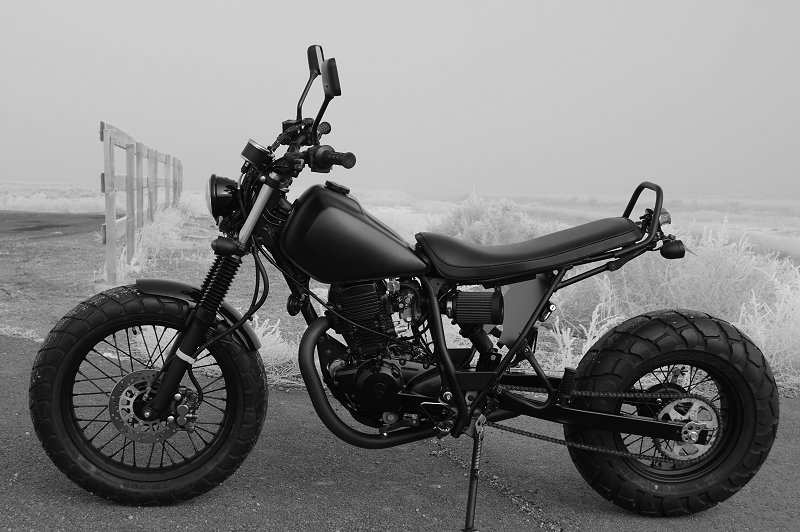
\includegraphics[width=\textwidth]{motor_original.png} \caption{Original image} %\label{fig:LPF} 
\end{subfigure}
\begin{subfigure}[b]{0.4\textwidth} 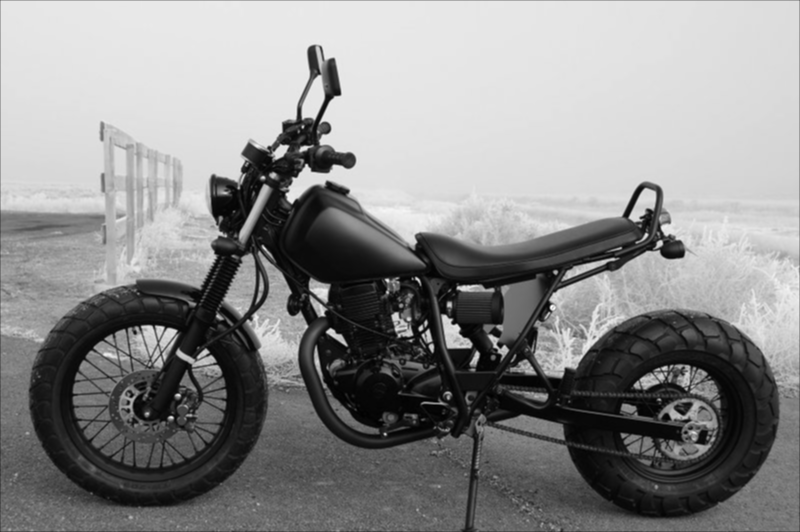
\includegraphics[width=\textwidth]{motor_direct.png} \caption{Low pass, direct}\end{subfigure}

\begin{subfigure}[b]{0.4\textwidth} 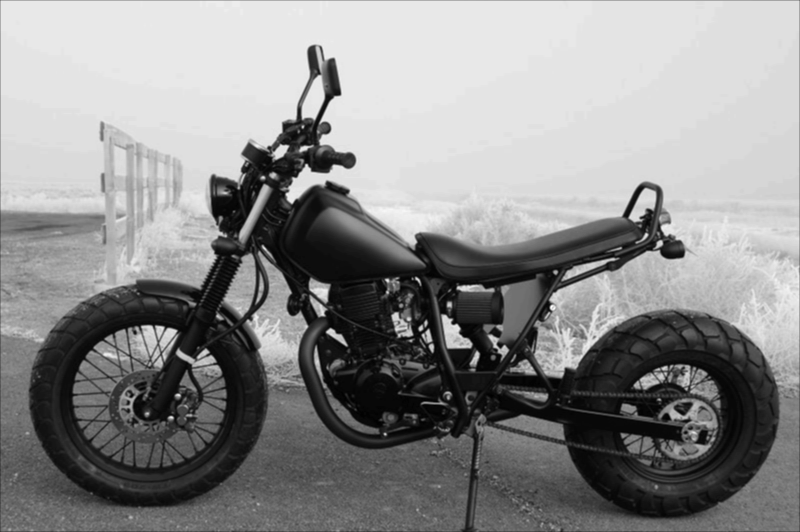
\includegraphics[width=\textwidth]{motor_lut_212.png} \caption{Low pass, LUT with $T_1$} %\label{fig:LPF} 
\end{subfigure}
\begin{subfigure}[b]{0.4\textwidth} 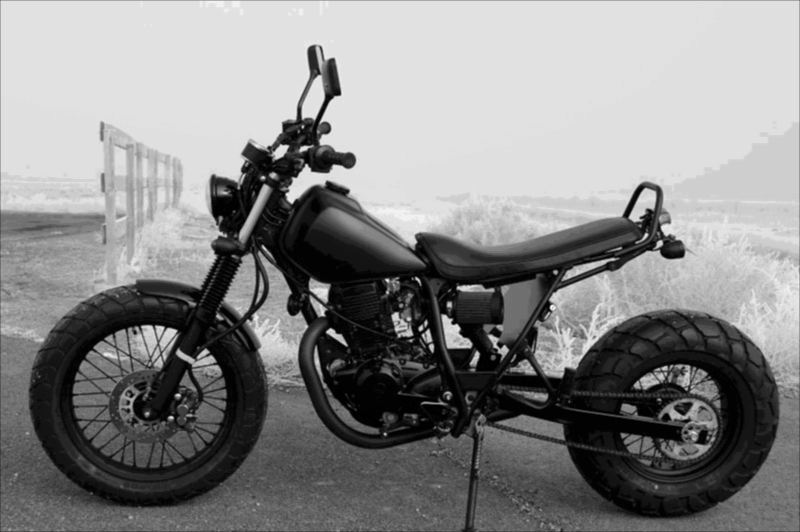
\includegraphics[width=\textwidth]{motor_lut_424.png} \caption{Low pass, LUT with $T_2$} \end{subfigure}
\caption{Comparison of filtered images. Figure A: The original image. Figure B: filtered image by direct applying kernel $K1$. Figure C: filtered image by using LUT with truncation scheme $T_1$. Figure D: filtered image by using LUT with truncation scheme $T_2$}
\label{fig:motor} 
\end{figure}


\begin{center}
\begin{table}
	 
    \begin{tabular}{ | c | c| c |}
    \hline
    Scheme & LUT Size & PSNR (dB) \\ \hline
    Direct & N/A & N/A  \\ \hline
    LUT with $T_1$ & 512KB & 41.8459 \\ \hline
    LUT with $T_2$ & 16KB & 30.4442 \\ \hline   
    \end{tabular}
    \bigskip
    
    \caption{Error and size of LUT for direct computation and LUTs with different truncation schemes.}
    \label{tbl:low_pass}
\end{table} 
\end{center}



The second numerical test involves the edge detection kernel (high pass kernel)
$$
K_2=\frac{1}{8}
\begin{bmatrix}
-1 & -1 & -1\\
-1 &  8 & -1\\
-1 & -1 & -1
\end{bmatrix}
$$
\begin{center}
\begin{table}
	
    \begin{tabular}{ | c | c | c | }
    \hline
    LUT Size & Best Truncation & PSNR (dB) \\ \hline
    16Kb& $(0,b,0)$ with $b=(4,2,4)^T$ & 30.4442 \\ \hline
    32Kb& $(0,b,0)$ with $b=(3,3,3)^T$ & 33.3275 \\ \hline 
    64Kb& $(0,b,0)$ with $b=(3,2,3)^T$ & 35.5597 \\ \hline 
    256Kb& $(0,b,0)$ with $b=(2,2,2)^T$ & 39.4329 \\ \hline 
    \end{tabular}
    \bigskip
    
    \caption{Best truncation scheme for fixed-size LUT}
    \label{tbl:optimization}
\end{table} 
\end{center}

What this kernel does is to expose the edges of the pictures with white  color and the non-edges tend to be black. Evidently the rank of $K_2$ is 2 and we resort to the singular value decomposition approach for reduction of the look up table size. The decomposition is given by 
$$
K_2=U\Sigma V^T
$$
where
$$
U=
\begin{bmatrix}
 0.0971 & 0.7004 & -0.7071\\
-0.9905 & 0.1374 & 0\\
 0.0971 & 0.7004 & 0.7071
\end{bmatrix}
, \ \ \ \ \ \Sigma=
\begin{bmatrix}
1.0245 & 0 & 0\\
0& 0.2745 & 0\\
0 & 0 & 0
\end{bmatrix}
$$
and
$$
V=
\begin{bmatrix}
 0.0971 & -0.7004 & -0.7071\\
-0.9905 & -0.1374 & 0\\
 0.0971 & -0.7004 & 0.7071
\end{bmatrix}
$$

Four LUTs are needed since we need to deal with $u_1=(0.0971,-0.9905,0.0971)$, $u_2=(0.7004,0.1374,0.7004)$, $v_1=(0.0971,-0.9905,0.0971)$, $v_2=(-0.7004,-0.1374,-0.7004)$ separately. The increase in the number of LUTs causes the size of LUT to rise. Another factor that contributes to the increase in the LUT size is the singular vectors which may stretch the original values of each pixel. As in the low pass filter, we still use the two truncation schemes $T_1$ and $T_2$ and the image we use here has the size of $1024\times 768$. The filtered images with direct computation and truncated LUTs are shown in figure \ref{fig:house} while the errors in PSNR and the size of the LUTs are listed in Table \ref{tbl:high_pass}. 
Note that the size of LUTs are significantly larger than that of the rank 1 kernel $K_1$. We observe that the size with SVD is approximately 8 times, rather than 4, of the previous LUT for rank 1 case. The extra increase in the size is due to the stretching effect of singular vectors. However, by truncating more numbers of bits, such as the $T_2$ scheme, we can draw similar conclusions, as in the case of low pass filter, that our truncated LUTs with the SVD scheme provides satisfactory result while the size of the LUTs are kept acceptable in practice. 

\begin{figure}[h] \centering 
\begin{subfigure}[b]{0.4\textwidth} 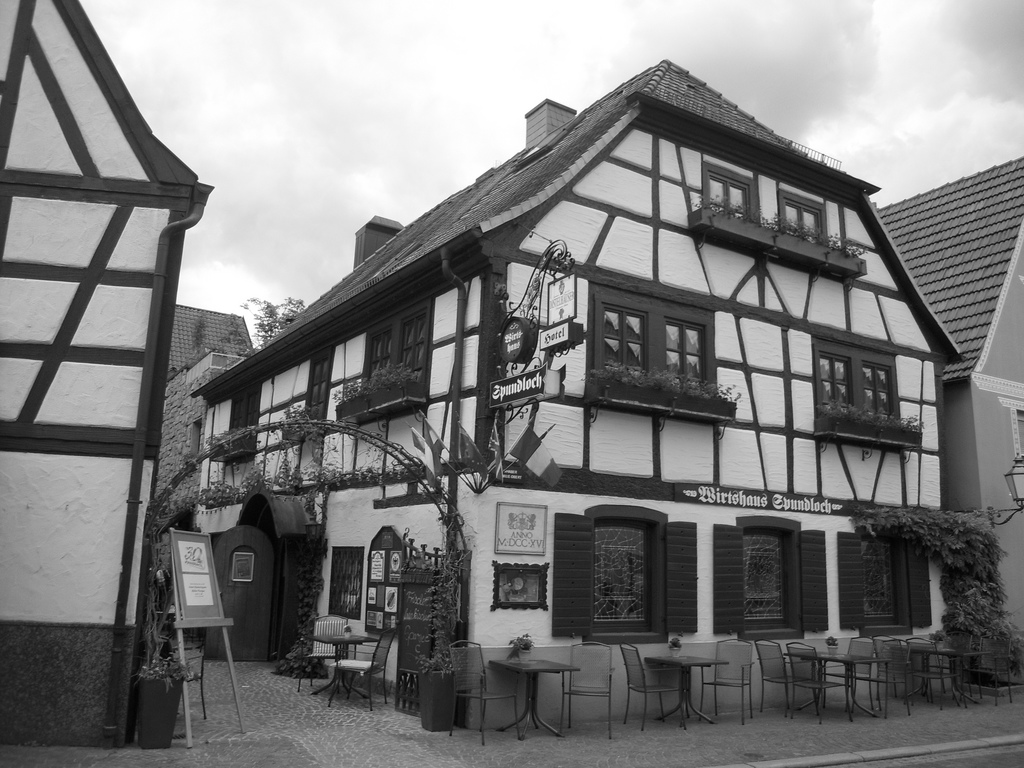
\includegraphics[width=\textwidth]{house_original.png} \caption{Original image} %\label{fig:LPF} 
\end{subfigure}
\begin{subfigure}[b]{0.4\textwidth} 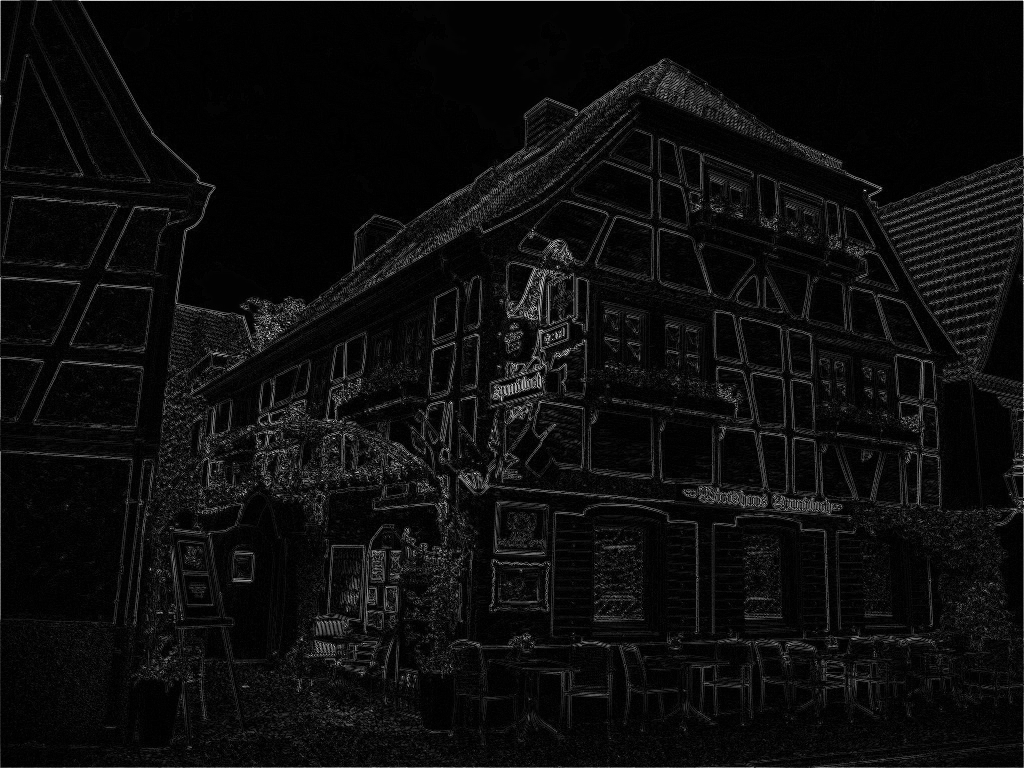
\includegraphics[width=\textwidth]{house_direct.png} \caption{Low pass, direct}\end{subfigure}

\begin{subfigure}[b]{0.4\textwidth} 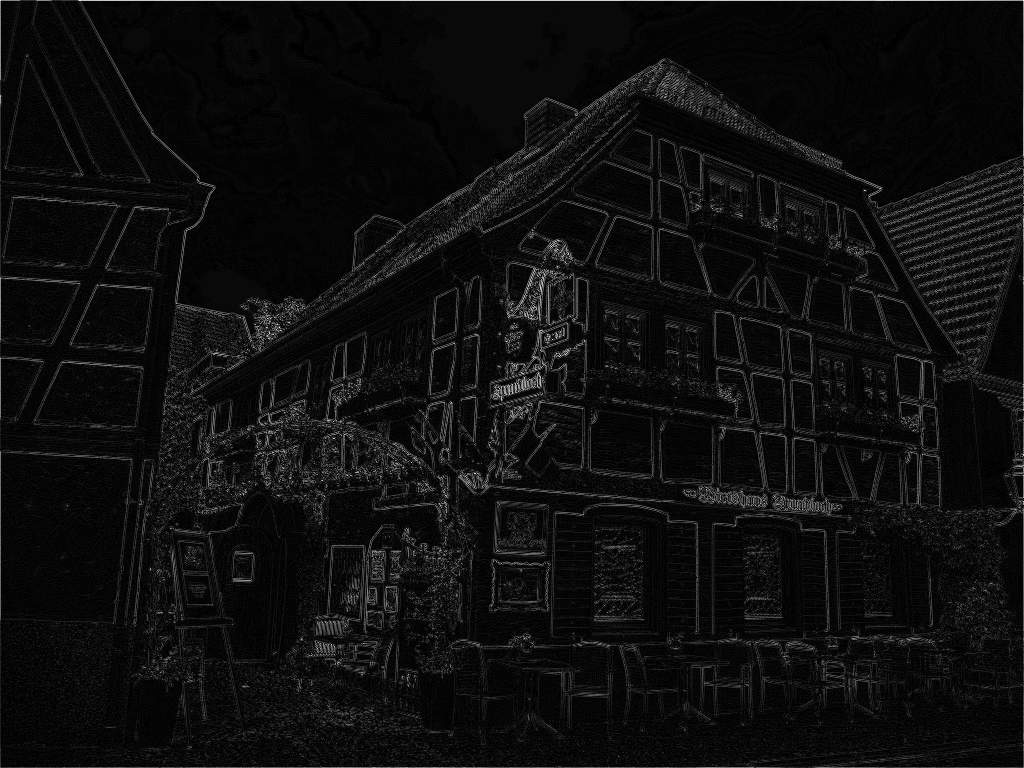
\includegraphics[width=\textwidth]{house_lut_212.png} \caption{Low pass, LUT with $T_1$} %\label{fig:LPF} 
\end{subfigure}
\begin{subfigure}[b]{0.4\textwidth} 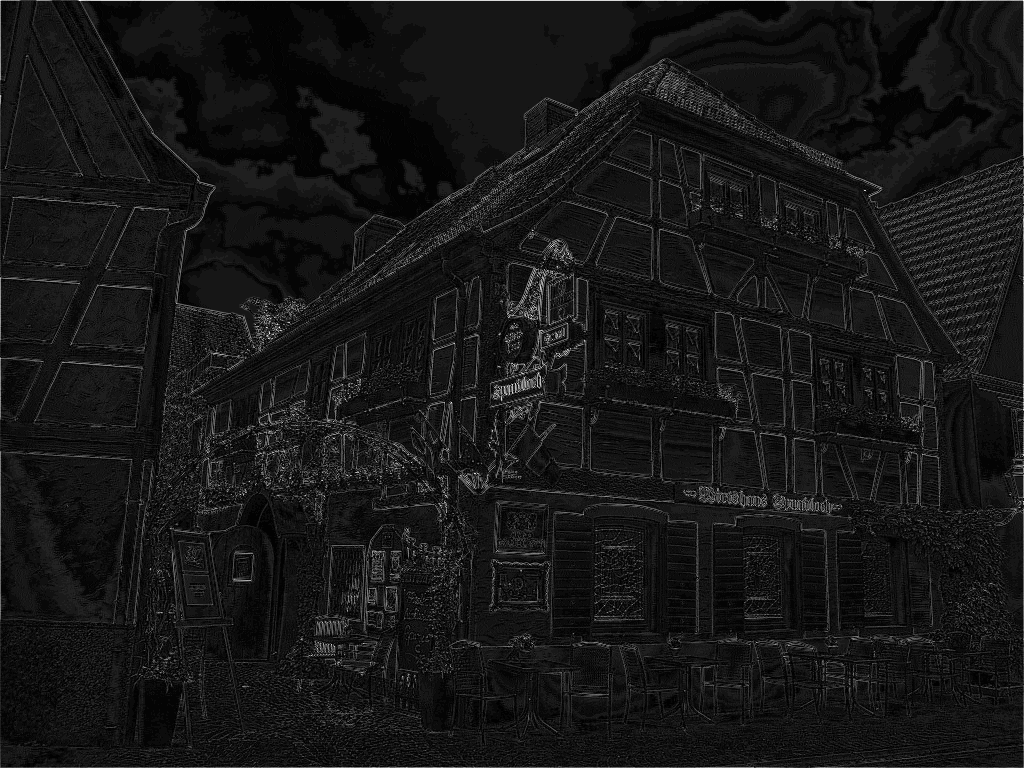
\includegraphics[width=\textwidth]{house_lut_424.png} \caption{Low pass, LUT with $T_2$} \end{subfigure}
\caption{Comparison of filtered images. Figure A: The original image. Figure B: filtered image by direct applying kernel $K2$. Figure C: filtered image by using LUT with truncation scheme $T_1$. Figure D: filtered image by using LUT with truncation scheme $T_2$}
\label{fig:house} 
\end{figure}



\begin{center}
\begin{table}
	 
    \begin{tabular}{ | c | c| c |}
    \hline
    Scheme & Total LUT Size & PSNR (dB) \\ \hline
    Direct & N/A & N/A  \\ \hline
    LUT with $T_1$ & 3.8MB & 40.9868 \\ \hline
    LUT with $T_2$ & 128.8KB & 30.4436 \\ \hline   
    \end{tabular}
    \bigskip
    
    \caption{Error and size of LUT for direct computation and LUTs with different truncation schemes.}
     \label{tbl:high_pass}
\end{table}
\end{center}


%====================================================
%A Decomposition Approx
%====================================================

\subsection{A Decomposition Approximation}
Recall that a rank 1 decomposition of our kernal $K$ had the form $$
K=b*c^T
$$
where $c,b \in \mathbb{R}^n$. This resulted in two LUTs of size $2^{24}$ bytes instead of the full LUT of size $2^{72}$ bytes. This drastically reduces the size of the LUT before any truncation but it requires us to have a rank 1 kernal $K$. What can we do for a filter that is not rank 1?
\\
\textbf{Question: Can we decompose the filter $K$ in a better way?}
\\
Consider the decomposition of our $(3\times 3)$ filter $K$ into the convolution:
$$K=A*B$$
where $A$ and $B$ are of the form


$$
A
=
\begin{bmatrix}
a & b & 0\\
c & d & 0\\
e & f & 0
\end{bmatrix}
,
B=
\begin{bmatrix}
g & h & i\\
j & k & l\\
0 & 0 & 0
\end{bmatrix}$$
\\
The main reason we would like a decomposition of this form is that due to the number of 0 entries in $A$ and $B$ we can automatically reduce the size of our full LUT of $2^{72}$ bytes to two LUTs of size $2^{48}$ bytes. In general this decomposition is not possible but we may be able to find an approximate decomposition by posing this as a minimization problem. The problem is 
$$\min \|K-A*B\|_F$$
\\
Notice that that are other ways we can arrange the variables $a,b,..,l$ in the matrices $A$ and $B$. There are in fact 9 choose 6 possibilities for each of the two matrices. This gives us a total of  $C(9,6)^2 =84^2= 7056$ possible minimization problems to solve. This seems like quite a lot of computation but this problem will actually be part of pre-processing. It is important to note the the minimizing values $(a,b,c,...,k,l)$ may be 0 and so we may further reduce LUT size. For example, the decomposition may lead to $A$ having only 2 nonzero entries and $B$ 4 nonzero entries. This would lead to two LUTs of size $2^{16}$ and $2^{32}$ bytes respectively.
\\
\\We can actually change the structure of the matrices $A$ and $B$ above to have a variable amount of nonzero entries in them. This will allow us to force more entries in the matrices to be zero resulting in smaller LUTs. 
\\
\textbf{Note:} After solving all possible minimization problems for a particular decomposition we will have a vector \textit{$f_{min}$} and a matrix \textit{$x_{min}$} containing all the min function values and minimizers. To get the ``best'' decomposition we look at the smallest function value. Since this will be an approximate decomposition we should look at all function values under a threshold and find the corresponding minimizers with the most number of zeros. For example there may be two function min values smaller than $\min(f_{min}) + 10^{-2}$ with minimizers $x_1=(1, 3, 0, 4, 2, 1)$ and $x_2=(0, 0, 0, 1, 2, 0)$. In this example we should choose the minimizer $x_2$ because it has more zeros in it. It should also be noted that minimizers may have very small values that may be truncated. 
\\
\\Ran an algorithm using fmin

$$
\begin{bmatrix}
-1 & -1 & -1\\
-1 & 8 & -1\\
-1 & -1 & -1
\end{bmatrix}
=
\begin{bmatrix}
a & d & 0\\
b & e & 0\\
c & f & 0
\end{bmatrix} *
\begin{bmatrix}
g & h & i\\
j & k & \ell \\
0 & 0 & 0
\end{bmatrix}
$$

$
A =
\begin{bmatrix}
  -0.372739294911747  &-0.443690961374357 & -0.457110102971229\\
  -0.509997537573061  & 2.683304035822869 &                  0\\
                   0  &                 0 &                  0
\end{bmatrix}
$

$
B =
\begin{bmatrix}
                   0&                   0&                   0\\
                   0&   2.681646089142412&  -0.509741093569434\\
  -0.456856367067759&  -0.443428387610633&  -0.372501463359094
\end{bmatrix}
$

\text{conv2(A,B,'same')}\\
$
\begin{bmatrix}
  -0.999554872469786  &-0.999821595552767  &-0.999640004082445\\
  -0.999646676848929  & 8.000063237563769  &-0.999819205287410\\
  -0.999737147772875  &-0.999878353018540  &-0.999534679981381
  \end{bmatrix}
$
  
  norm(F-conv2(A,B,'same'),'fro')

ans =

     $9.063656510413503e-04$

%\section{Further Questions}

\section{Thursday August 6: Daily Notes}
\subsection{Compute an algorithm using a look-up table for a high-pass kernel matrix} 
$\frac{1}{8}
\begin{bmatrix}
0 & -1 & 0\\
-1 & 4 & -1\\
0 & -1 & 0
\end{bmatrix}$ using a truncation technique using truncation matrix
$\begin{bmatrix}
8 &4 &8\\
4 &2 &4\\
8 &4 &8
\end{bmatrix}$. This particular look-up table was created in about 15-19 seconds.

\subsection{
Compare results of linear filters on Matlab with and without truncating digits}
Truncating with the following truncating matrices look acceptable for gray-scale images:
$
T_0=
\begin{bmatrix}
0 &4 &0\\
4 &0 &4\\
0 &4 &0
\end{bmatrix},
T_1=
\begin{bmatrix}
0 &4 &0\\
4 &1 &4\\
0 &4 &0
\end{bmatrix}
T_2=
\begin{bmatrix}
0 &4 &0\\
4 &2 &4\\
0 &4 &0
\end{bmatrix}
T_3=
\begin{bmatrix}
0 &5 &0\\
5 &3 &5\\ 
0 &5 &0
\end{bmatrix}
T_4=
\begin{bmatrix}
0 &3 &0\\
3 &1 &3\\
0 &3 &0
\end{bmatrix}
.$

A normalized gradient magnitude from Sobel-Feldman operator \cite{Wikipedia/Sobel}
$\mathbf{G} = \sqrt{ {\mathbf{G}_x}^2 + {\mathbf{G}_y}^2 }$

where

$\mathbf{G}_x = \begin{bmatrix} 
 -1 & 0 & +1  \\
-2 & 0 & +2 \\
-1 & 0 & +1 
\end{bmatrix} * \mathbf{A}
\quad
\mbox{and}
\quad   
\mathbf{G}_y = \begin{bmatrix} 
-1 & -2 & -1 \\
 0 & 0 & 0 \\
+1 & +2 & +1
\end{bmatrix} * \mathbf{A}$.

Here * denotes the 2-dimensional convolution operation.

Some high-pass kernel matrices:
\begin{itemize}
\item
$
\frac{1}{8}
\begin{bmatrix}
0 & -1 & 0\\
-1 & 4 & -1\\
0 & -1 & 0
\end{bmatrix}$
\item
$
\frac{1}{8}
\begin{bmatrix}
-1 & -1 & -1\\
-1 & 8 & -1\\
-1 & -1 & -1
\end{bmatrix}$
\end{itemize}

A low-pass kernel matrix:
\begin{itemize}
\item
$
\frac{1}{16}
\begin{bmatrix}
1 & 2 & 1\\
2 & 4 & 2\\
1 & 2 & 1
\end{bmatrix}$
\end{itemize}

A Scharr Gradient kernel matrix:
\begin{itemize}
\item
$
\frac{1}{32}
\begin{bmatrix}
3 & 10 & 3\\
0 & 0 & 0\\
-3 & -10 & -3
\end{bmatrix}$
\end{itemize}

An unsharp mask kernel filter:
\begin{itemize}
\item
$
\frac{1}{8}
\begin{bmatrix}
0 &-\lambda &0\\
-\lambda &1-0.3*\lambda &-\lambda\\
0 &-\lambda &0
\end{bmatrix}
$
where $\lambda=0.1$.
\end{itemize}
%%=================================


\begin{thebibliography}{widest entry}
\bibitem[WSLQE06]{WSLQE06}
Wu, C. W., Stanich, M., Li, H., Qiao, Y., Ernst, L., "Fast Error Diffusion and Digital Halftoning Algorithms Using Look-up Tables," Proceedings of NIP22: International Conference on Digital Printing Technologies, Denver, Colorado, pp. 240-243, September 2006.


\bibitem[Wikipedia/Sobel]{Wikipedia/Sobel}
{Sobel operator}%{https://en.wikipedia.org/wiki/Sobel_operator}
\bibitem[wikipedia/PSNR]{wikipedia/PSNR}{PSNR(Peak Signal-to-Noise Ratio)}

\bibitem[FWZ05]{FWZ05}
Jufu Feng, Liwei Wang, Yan Zhang, "On the Euclidean Distance of Images," IEEE Transactions on Pattern Analysis and Machine Intelligence, vol. 27, no. 8, pp. 1334-1339, 2005.
\end{thebibliography}
 \end{document}